%!TEX root = ../Masterarbeit.tex
\chapter{Ergebnis}
\label{cha:ergebnis}
Im Folgenden wird der Funktionsumfang und die Anwendung der Web-Applikation beschrieben.

\section{Anwendung}
\subsection{Eingeben eines Suchbegriffes}
In Abbildung \ref{fig:screenHome} ist die Web-Applikation in ihrer Ausgangssituation zu sehen. Der Nutzer kann mit einem Klick auf die Selectbox (\glqq Choose a timeframe!\grqq) einen Suchbegriff eingeben. Die Eingabem�glichkeiten, deren Quelle und der jeweils daraus resultierende Zeitpunkt, der f�r die Suche relevant ist, sind in der Tabelle \ref{tab:eingabeformen} aufgef�hrt.

\begin{table}
    \begin{tabular}{|l|P{7cm}|l|}
	\hline
	Eingabe 			& Suchvorschlag & Zeitpunkt \\ \hline \hline
	Filmtitel			& Filmtitel von \textbf{Rotten Tomatoes} und \textbf{IMDb} 	& Filmstart \\ \hline
	Musiktitel 			& Musiktitel von \textbf{MusicBrainz}  						& Ver�ffentlichungsdatum \\  \hline
	Interpret			& Musiktitel des K�nstlers, die auf \textbf{MusicBrainz} zu finden sind  		& Ver�ffentlichungsdatum \\
	\hline
	\end{tabular}
	\caption{Eingabeformen, m�gliche Quellen und das jeweils aufgel�ste Datum}\label{tab:eingabeformen}
\end{table}

Um unn�tige Requests zu vermeiden, wird erst bei Eingabe des dritten Zeichens eine Suche gestartet. In Abbildung \ref{fig:screenSuggestions} ist die Anzeige von Suchvorschl�gen zu sehen. Anhand des Icons ist zu erkennen, von welcher Quelle der Suchvorschlag kommt. Soweit vorhanden, wird daneben ein Thumbnail des Filmplakats angezeigt, sollte keines gefunden worden, wird ein Platzhalter angezeigt. Au�erdem werden Titel der vorgeschlagenen Items, sowie das jeweilige Erscheinungsjahr angezeigt. Das Jahr bezeichnet den Zeitraum, der durchsucht wird, wenn der Nutzer darauf klickt.

\begin{figure}[htb]
	\begin{center}
		\shadowimage[width=14cm]{screenHome.png}
		\caption{Screenshot des Homescreens}
		\label{fig:screenHome}
	\end{center}
\end{figure}


\begin{figure}[htb]
	\begin{center}
		\shadowimage[width=14cm]{screenSuggestionsGood.png}
		\caption{Screenshot der Anzeige der Suchvorschl�ge}
		\label{fig:screenSuggestions}
	\end{center}
\end{figure}

\begin{figure}[htb]
	\begin{center}
		\shadowimage[width=14cm]{screenSuggestionFerris.png}
		\caption{Screenshot der Anzeige der Detailansicht der Suchanfrage}
		\label{fig:screenSearchDetail}
	\end{center}
\end{figure}


\subsection{Pr�sentation des Suchergebnisses}
In Abbildung \ref{fig:screenSearchResults} ist die Anzeige der Suchergebnisse f�r das Jahr 1990 zu sehen. Im Hauptbereich sind alle Filmplakate zu sehen, die beim Scrapen der \textbf{IMDb}-Seite f�r das Jahr gefunden und dessen Daten �ber die \textbf{Rotten Tomatoes}-API vervollst�ndigt werden. Im rechten Drittel der Anzeige ist die Liste der gefundenen Trailer von der API \textbf{TrailerAddict} zu sehen. Diese sind jeweils in IFrames eingebettet und k�nnen unabh�ngig voneinander abgespielt werden.\footnote{Auf dem Screenshot \ref{fig:screenSearchResults} wird der Trailer zu \glqq Robocop II\grqq \ abgespielt. (Erster Eintrag in der Player-Ansicht.)}

\subsection{Ansicht zus�tzlicher Informationen eines Ergebnis-Items}
F�hrt man mit dem Mauszeiger �ber ein Item \zB ein Filmplakat, erscheinen drei Icons, �ber die weitere Aktionen, die das Item betreffen, durchgef�hrt werden k�nnen.\footnote{Die Hover-Ansicht ist in Abbildung \ref{fig:screenSearchResults} am Beispiel des Filmes \glqq Rocky V\grqq \ zu sehen. (Erste Reihe, 3. v.l.)}

\paragraph{Informations-Icon} Dieses Icon dient der Anzeige des Item-Titels, sowie den Namen des Dienstes, von dem dieses Item bezogen wurde. Ebenfalls werden der Medien-Typ und Medien-Subtyp angezeigt.

\paragraph{Link-Icon} �ber das Link-Icon kann der Nutzer direkt zur URL des gew�hlten Items navigieren. Im Falle eines Filmes, der auf \textbf{Rotten Tomatoes} gefunden wurde, wird die Detailseite des Filmes auf der \textbf{Rotten Tomatoes}-Website in einem neuen Tab ge�ffnet.

\paragraph{Plus-Icon} Das Plus-Icon verf�gt zu diesem Zeitpunkt �ber keine Funktion, soll in Zukunft jedoch die Funktion bieten, falls es sich bei dem Item um abspielbaren Inhalt handelt, dieses zur Playlist-Queue hinzuzuf�gen.

\begin{figure}[htb]
	\begin{center}
		\shadowimage[width=14cm]{screenSearchResults1990.png}
		\caption{Screenshot der Anzeige der Suchergebnisse des Jahres 1990}
		\label{fig:screenSearchResults}
	\end{center}
\end{figure}

\subsection{Anzeige der Suchdetails}
Nach dem Durchf�hren einer Suche, kann �ber das Menu-Icon, welches sich neben dem Suche-Eingabefeld befindet, das Menu aufgerufen werden. Wie in Abbildung \ref{fig:screenSearchDetail} zu sehen ist, werden unter \glqq Search Details\grqq \ das gesuchte Jahr, der Titel des gesuchten Items, sowie der Medien- und Medien-Subtyp angezeigt. Au�erdem wird, soweit vorhanden, ein repr�sentatives Bild angezeigt, in diesem Fall das Filmplakat von \glqq Ferris Bueller\grq s Day off\glqq . �ber den Link der Quelle, in der Abbildung \glqq RottenTomatoes\grqq , kann auf die Webseite des jeweiligen Items auf der Dienstseite navigiert werden. Die Option \glqq Filter Result\grqq \ dient zu diesem Zeitpunkt lediglich als Platzhalter f�r die zuk�nftige Funktion des Filterns des Ergebnisses.


\subsection{Funktionalit�t des Players}
Derzeit wird der Player lediglich mit Film-Trailern bef�llt. Die Funktionalit�t des Players konnte nicht implementiert werden, da die \textbf{TrailerAddict}-API lediglich das Einbetten ihrer Trailer vorsieht. Dementsprechend ist das Result, welches von dieser API zur�ckkommt, ein HTML-Snippet, das in einem IFrame in \arbeitstitel \ eingebettet wird. Eine externe Steuerung von IFrames, sodass die Player-Funktionalit�t, wie das Abspielen, Skippen oder Pausieren eines Trailers nicht �ber die Player-Buttons von \arbeitstitel \ nicht bewerkstelligt werden kann.

\section{\arbeitstitel -API}
Durch das \textbf{Express}-Framework ist die implementierte Funktionalit�t ebenfalls als RESTful-API verwendbar. Zu einer Einbindung der API werden die Routen \lstinline{/suggestions} und \lstinline{/search} bereitgestellt. In den Abbildungen \ref{fig:suggestionAPI} und \ref{fig:resultItemAPI} sind die Dokumentationen der beiden Funktionen zu sehen.\footnote{Bei den Abbildungen \ref{fig:suggestionAPI} und \ref{fig:resultItemAPI} handelt es sich jeweils um Screenshots der mit dem Apiary Framework \citep{apiary} erstellten \arbeitstitel -Dokumentation.}



\begin{figure}[htb]
	\begin{center}
		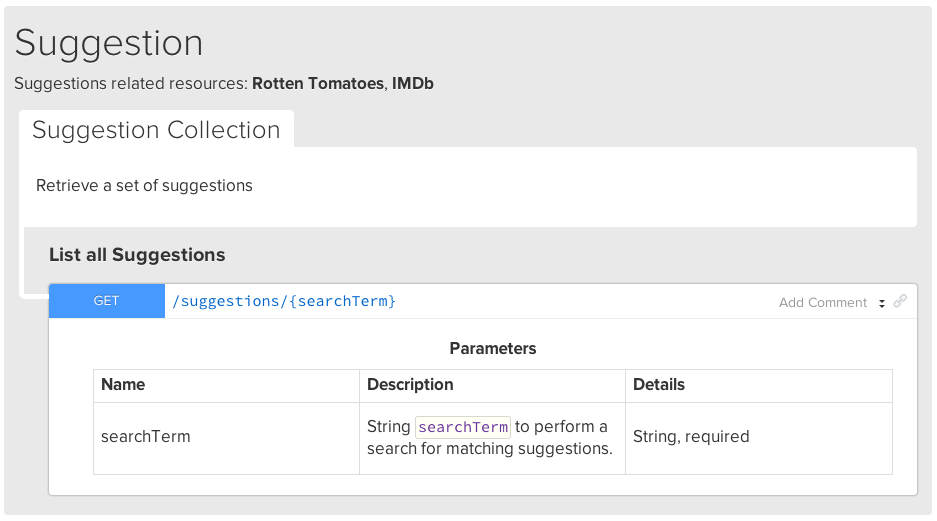
\includegraphics[width=1\textwidth]{suggestionAPI.png}
		\caption{API-Entit�t Suggestion}
		\label{fig:suggestionAPI}
	\end{center}
\end{figure}

\begin{figure}[htb]
	\begin{center}
		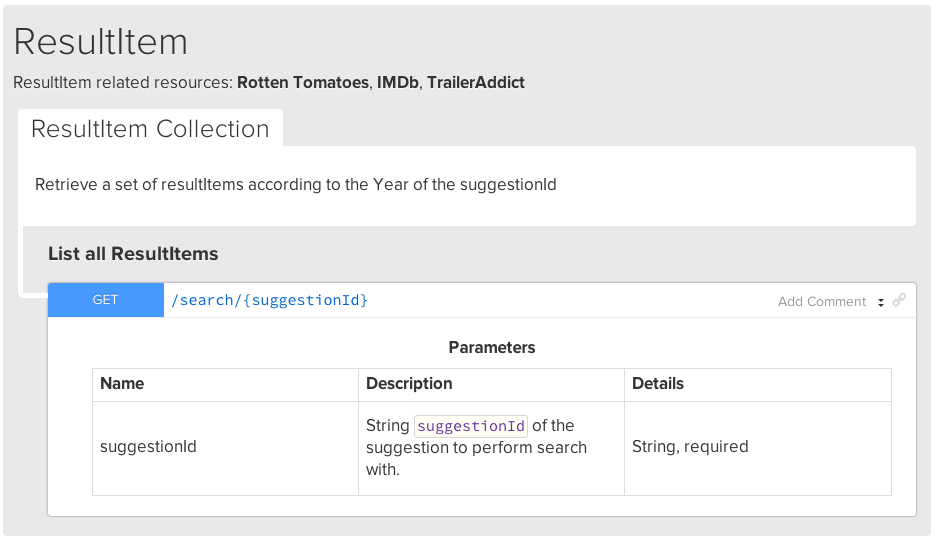
\includegraphics[width=1\textwidth]{resultItemAPI.png}
		\caption{API-Entit�t ResultItem}
		\label{fig:resultItemAPI}
	\end{center}
\end{figure}

% \todo{sch�ner formatieren}
% \begin{itemize}
% 	\item \lstinline{GET /suggestions}
% 	\begin{itemize}
% 		\item Liefert eine Liste an Suchvorschl�gen anhand eines Suchbegriffes
% 		\item \textbf{params}: \texttt{String:searchterm}
% 		\item \textbf{returnValue}: \texttt{List<suggestion>}
% 	\end{itemize}
% 	\item \lstinline{GET /search}
% 	\begin{itemize}
% 		\item Liefert eine Liste an Suchergebnissen anhand eines Suchbegriffes
% 		\item \textbf{params}: \texttt{String:suggestionId}
% 		\item \textbf{returnValue}: \texttt{List<resultItem>}
% 	\end{itemize}
% \end{itemize}
